\documentclass{beamer}
\usepackage[UKenglish]{babel}
\usepackage[UKenglish]{isodate}
\usepackage{graphicx}
\usepackage{tikz}
\usepackage{bm}
\usepackage{bbm}
\usepackage{mathtools}
\usepackage[bibstyle=ieee,citestyle=authoryear]{biblatex}
\usepackage{setspace}
\usepackage{csvsimple}
\usepackage{pgfplots}
\usepackage{xcolor}
\usetikzlibrary{shapes,bayesnet,arrows.meta,arrows,calc,pgfplots.colormaps}

% TODO: Avoid saying that epsilon is arbitrary and using phrases like 'sufficiently
% small', i.e., update theorems, make sure they match the paper
% TODO: could add the example (figure and notation)
% TODO: could add the algorithm (maybe should?)


\definecolor{myblue}{HTML}{0000FF}
\definecolor{myred}{HTML}{FF0000}
\definecolor{mybrown}{HTML}{734C26}
\definecolor{mybluetwo}{HTML}{0072BD}
\definecolor{myyellow}{HTML}{EDB120}
\definecolor{myredtwo}{HTML}{D95319}

\addbibresource{talk.bib}
\usetheme{Frankfurt}
\beamertemplatenavigationsymbolsempty
\newtheorem{proposition}{Proposition}

% Makes the legend have a single rectangle per colour
\pgfplotsset{
  /pgfplots/ybar legend/.style={
    /pgfplots/legend image code/.code={%
      \draw[##1,/tikz/.cd,bar width=3pt,yshift=-0.2em,bar shift=0pt]
      plot coordinates {(0cm,0.8em)};},
  },
}

\DeclareMathOperator*{\argmax}{arg\,max}
\DeclareMathOperator{\diag}{diag}
\DeclareMathOperator{\tr}{tr}
\newcommand{\Kuu}{\mathbf{K}_{\mathbf{u},\mathbf{u}}}
\newcommand{\Krr}{\mathbf{K}_{\mathbf{r},\mathbf{r}}}
\newcommand{\Kru}{\mathbf{K}_{\mathbf{r},\mathbf{u}}}
\newcommand{\rinf}{\lVert \mathbf{r} \rVert_\infty}
\newcommand{\vbound}{\frac{\rinf + \log|\mathcal{A}|}{1 - \gamma}}
\newcommand{\dt}{\frac{\partial}{\partial t}}
\newcommand{\dx}{\,d\mathbf{r}\,d\mathbf{u}}
\newcommand{\V}{V_{\mathbf{r}}}
\newcommand{\pione}{\pi(a_1 \mid s_1)}
\newcommand{\pitwo}{\pi(a_1 \mid s_2)}
\newcommand{\pithree}{\pi(a_2 \mid s_3)}

\renewcommand{\thempfootnote}{\arabic{mpfootnote}}
\DeclarePairedDelimiterX{\infdivx}[2]{(}{)}{%
  #1\;\delimsize\|\;#2%
}
\newcommand{\DKL}{D_{\mathrm{KL}}\infdivx}

\author{Paulius Dilkas}
\title{Variational Inference for Inverse Reinforcement Learning with Gaussian
  Processes}
%\date{15th January 2019} % TODO

\begin{document}

\maketitle

\section{Introduction}

\begin{frame}
  \begin{overprint}
    \onslide<1>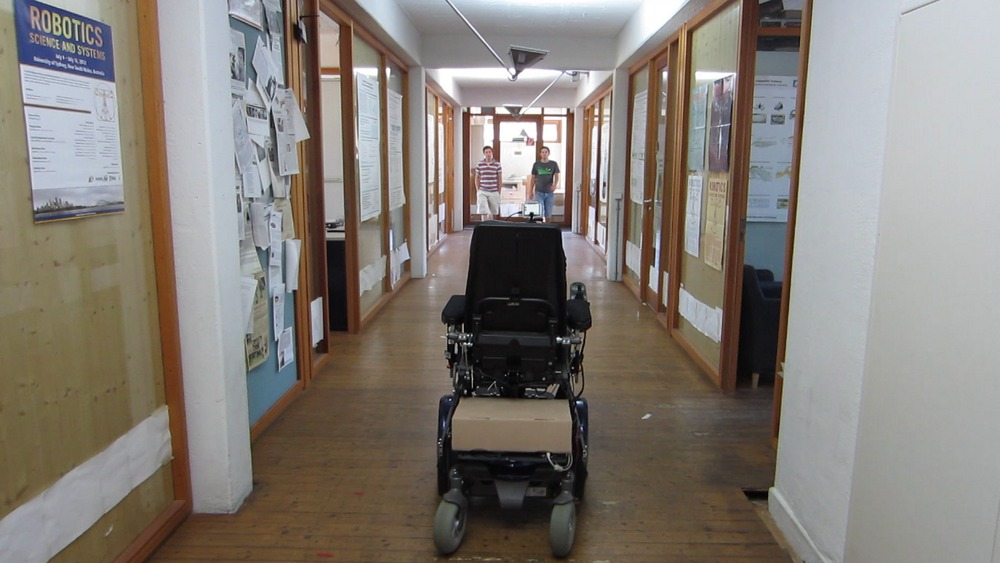
\includegraphics[width=\textwidth]{images/image-044.jpg}
    \onslide<2>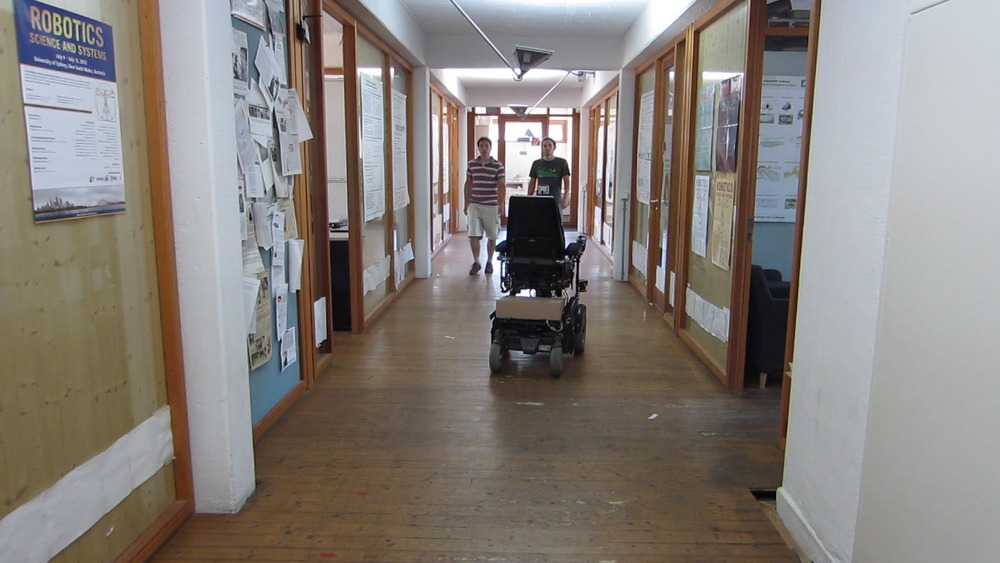
\includegraphics[width=\textwidth]{images/image-045.jpg}
    \onslide<3>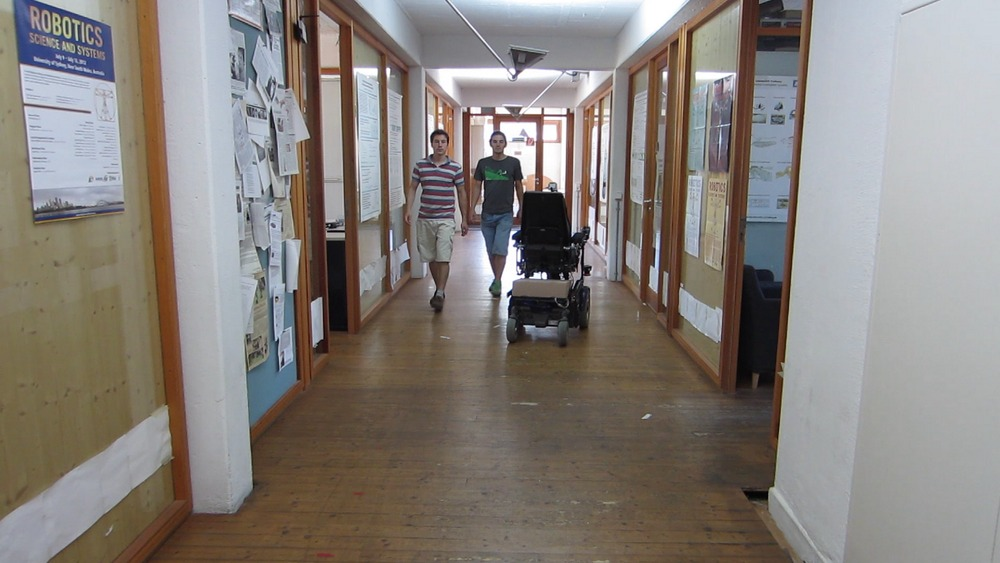
\includegraphics[width=\textwidth]{images/image-048.jpg}
    \onslide<4>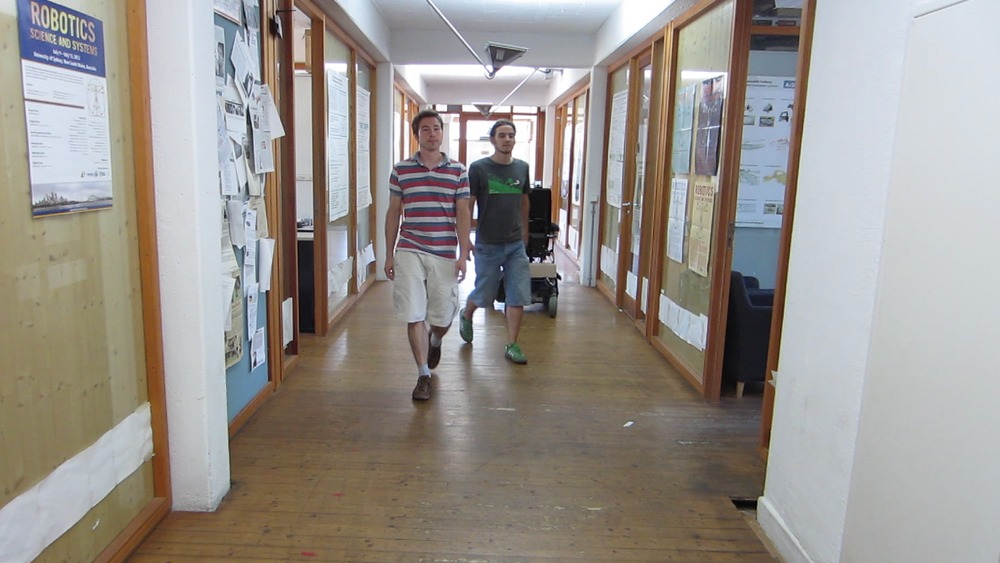
\includegraphics[width=\textwidth]{images/image-049.jpg}
  \end{overprint}
  \begin{spacing}{0.5}
    {\tiny\color{gray}\fullcite{DBLP:journals/ijrr/KretzschmarSSB16}}
  \end{spacing}
\end{frame}

\begin{frame}{Inverse Reinforcement Learning (IRL)}
  \begin{columns}
    \begin{column}{0.2\textwidth}
      Model (MDP)
      \begin{figure}
        \centering
        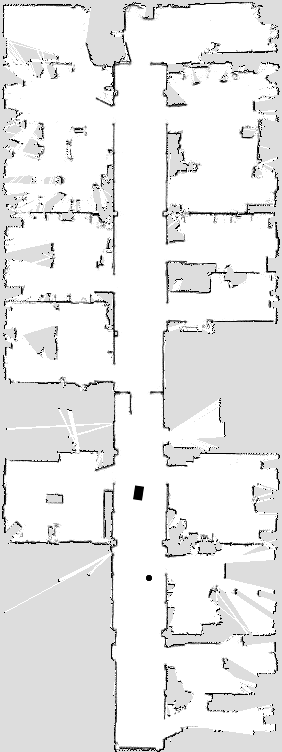
\includegraphics[width=\textwidth]{images/image-052.png}
      \end{figure}
    \end{column}
    \begin{column}{0.8\textwidth}
      Demonstrations
      \begin{figure}
        \centering
        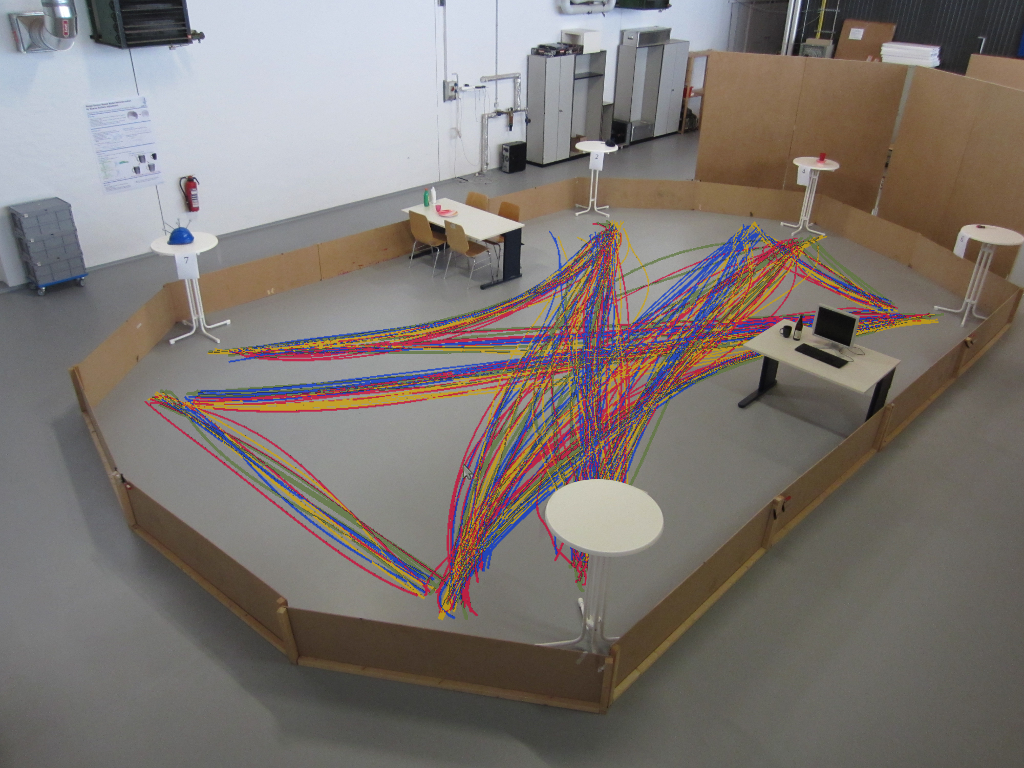
\includegraphics[width=\textwidth]{images/image-013.png}
      \end{figure}
    \end{column}
  \end{columns}
  \begin{spacing}{0.5}
    {\tiny\color{gray}\fullcite{DBLP:journals/ijrr/KretzschmarSSB16}}
  \end{spacing}
\end{frame}

\begin{frame}
  \begin{definition}[Markov Decision Process]
    An MDP is a set $\mathcal{M} = \{\mathcal{S}, \mathcal{A}, \mathcal{T},
    \gamma, \mathbf{r} \}$ that consists of:
    \begin{itemize}
    \item states $\mathcal{S}$
    \item actions $\mathcal{A}$
    \item transition function $\mathcal{T} : \mathcal{S} \times \mathcal{A}
      \times \mathcal{S} \to [0, 1]$
    \item discount factor $\gamma \in [0, 1)$
    \item reward function/vector $\mathbf{r} \in \mathbb{R}^{|\mathcal{S}|}$ (or
      $r : \mathcal{S} \to \mathbb{R}$)
    \end{itemize}
  \end{definition}
  \pause
  \begin{definition}[Inverse Reinforcement Learning \parencite{DBLP:conf/colt/Russell98}]
    Given:
    \begin{itemize}
    \item $\mathcal{M} \setminus \{ \mathbf{r} \}$,
    \item demonstrations $\mathcal{D} = \{ \zeta_i \}_{i=1}^N$, where $\zeta_i =
      \{ (s_{i,t}, a_{i,t}) \}_{t=1}^T$,
    \item features $\mathbf{X} \in \mathbb{R}^{|\mathcal{S}| \times d}$,
    \end{itemize}
    find $\mathbf{r}$.
  \end{definition}
\end{frame}
% TODO: add motivation for IRL from the Turing talk

\begin{frame}{Other Applications}
  \begin{columns}
    \begin{column}{0.5\textwidth}
      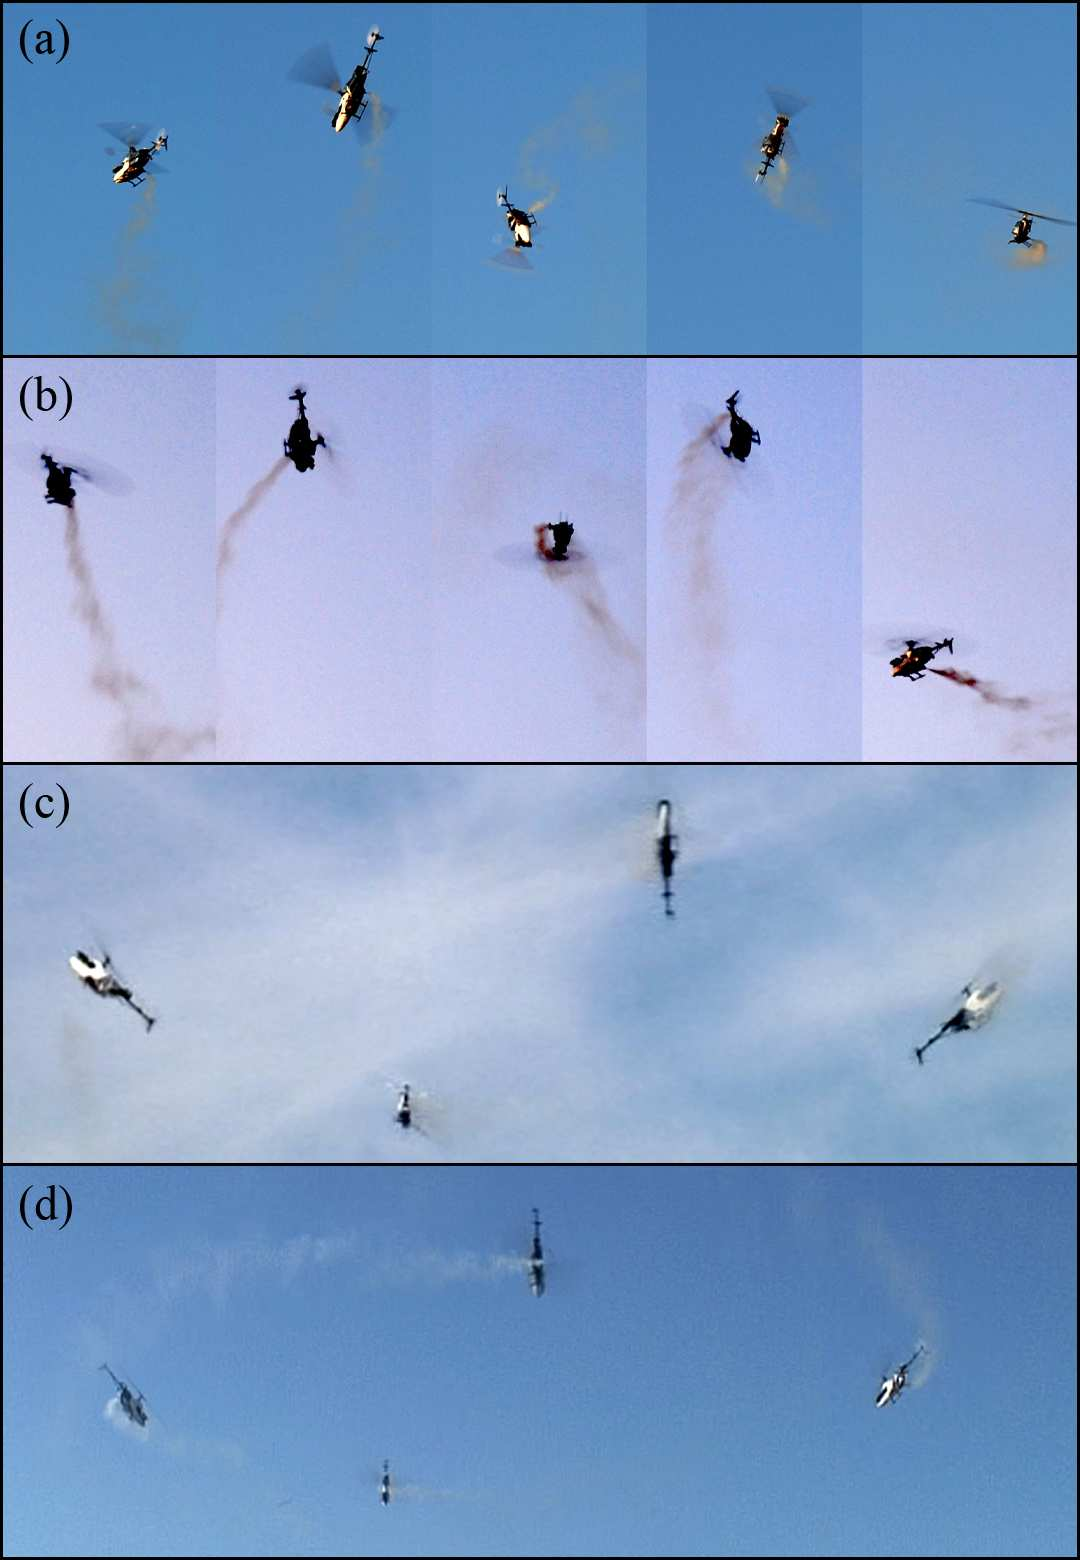
\includegraphics[height=0.8\textheight]{images/helicopter-000.jpg}
      \begin{spacing}{0.5}
        {\tiny\fullcite{DBLP:conf/nips/AbbeelCQN06}}
      \end{spacing}
    \end{column}
    \begin{column}{0.5\textwidth}
      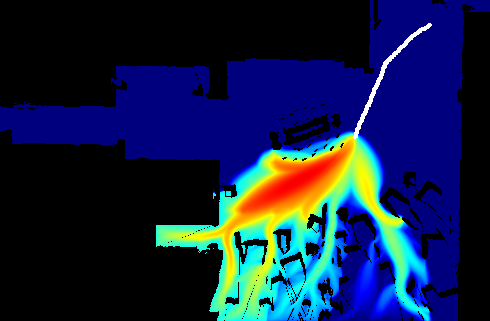
\includegraphics[width=0.5\textwidth]{images/pedestrians-013.png}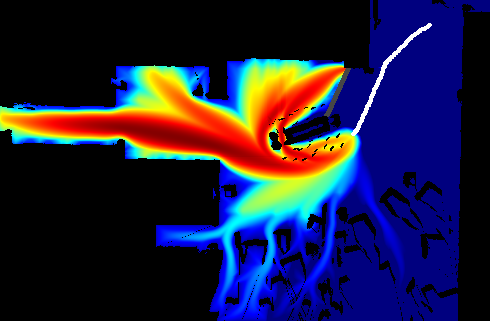
\includegraphics[width=0.5\textwidth]{images/pedestrians-014.png}
      \begin{spacing}{0.5}
        {\tiny\fullcite{DBLP:conf/iros/ZiebartRGMPBHDS09}}
      \end{spacing}
      \vspace{0.5cm}
      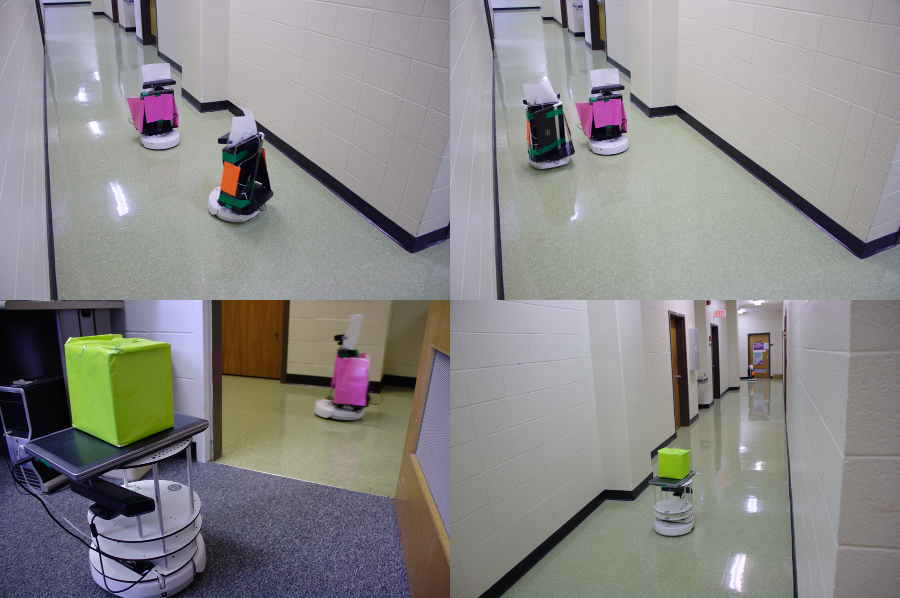
\includegraphics[width=\textwidth]{images/patrolling.png}
      \begin{spacing}{0.5}
        {\tiny\fullcite{DBLP:conf/atal/BogertD14}}
      \end{spacing}
    \end{column}
  \end{columns}
\end{frame}

\begin{frame}
  \begin{itemize}
  \item Has the model learned optimal behaviour?
  \item Can it recognise its own weak spots?
  \item Solution: variational inference (VI)
  \end{itemize}
  \begin{tikzpicture}[remember picture,overlay]
    \node at (9, 1) {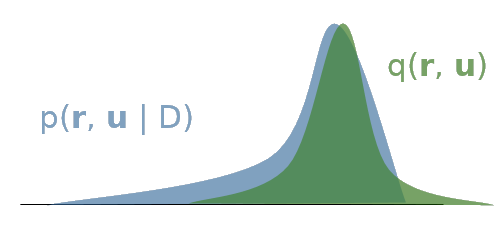
\includegraphics[scale=1]{images/vi.png}};
  \end{tikzpicture}
  \pause
  \begin{block}{Outline for the rest of the talk}
  \begin{itemize}
  \item Maximum causal entropy and stochastic policies
  \item Reward function as a Gaussian process (GP)
  \item Variational approximation of the posterior distribution
  \item Theoretical results: how can we compute the gradient?
  \item Empirical results: does it work?
  \item Further work: what comes next?
  \end{itemize}
  \end{block}
\end{frame}

\section{Entropy}

\begin{frame}{Maximum Causal Entropy}
  \begin{minipage}[t]{\textwidth}
    \begin{block}{Standard MDP}
      \[
        V_{\mathbf{r}}(s) \coloneqq r(s) + \gamma \max_{a \in \mathcal{A}}
        \sum_{s' \in \mathcal{S}} \mathcal{T}(s, a, s')V_{\mathbf{r}}(s')
      \]
    \end{block}
    \begin{block}{Maximum Causal Entropy MDP\textsuperscript{1}}
      \[
        V_{\mathbf{r}}(s) \coloneqq \log \sum_{a \in \mathcal{A}} \exp \left(
          r(s) + \gamma\sum_{s' \in \mathcal{S}} \mathcal{T}(s, a,
          s')V_{\mathbf{r}}(s') \right)
      \]
    \end{block}
    \vphantom{\footfullcite{DBLP:conf/icml/ZiebartBD10}}
    \vspace{1cm}
  \end{minipage}
\end{frame}

\section{GPs}

\begin{frame}{Reward Function as a Gaussian Process}
  \begin{block}{Automatic Relevance Determination Kernel}
    For any two states $\mathbf{x}_i, \mathbf{x}_j \in \mathbb{R}^d$,
    \[
      k_{\bm\lambda}(\mathbf{x}_i, \mathbf{x}_j) = \lambda_0\exp\left(
        -\frac{1}{2}(\mathbf{x}_i - \mathbf{x}_j)^\intercal\bm\Lambda(\mathbf{x}_i -
        \mathbf{x}_j) - \mathbbm{1}[i \ne j]\sigma^2\tr(\bm\Lambda) \right)
    \]
    where $\bm\Lambda = \diag(\lambda_1, \dots, \lambda_d)$, $\sigma^2 =
    10^{-2}/2$,
    \[
      \mathbbm{1}[b] = \begin{cases}
        1 & \mbox{if $b$ is true} \\
        0 & \mbox{otherwise}.
      \end{cases}
    \]
  \end{block}
\end{frame}

\begin{frame}{Reward Function as a Gaussian Process}
    \begin{block}{Inducing Points}
      \begin{itemize}
      \item $m \ll |\mathcal{S}|$ states,
      \item their features $\mathbf{X_u}$
      \item and rewards $\mathbf{u}$.
      \end{itemize}
    \end{block}

  \begin{block}{The GP Then Gives Gives...}
    \begin{itemize}
    \item Kernel/covariance matrices: $\Kuu$, $\Kru$, $\Krr$
    \item Prior probabilities:
      \begin{itemize}
      \item $p(\mathbf{u}) = \mathcal{N}(\mathbf{u}; \mathbf{0}, \Kuu)$
      \item $p(\mathbf{r} \mid \mathbf{u}) = \mathcal{N}(\mathbf{r};
        \Kru^\intercal\Kuu^{-1}\mathbf{u}, \Krr - \Kru^\intercal\Kuu^{-1}\Kru)$
      \end{itemize}
    \end{itemize}
  \end{block}
\end{frame}

\section{VI}

\begin{frame}{Variational Approximation}
  \begin{block}{Previous Work}
    \begin{itemize}
    \item Levine et al. (2011) assume that $\mathbf{r} =
      \Kru^\intercal\Kuu^{-1}\mathbf{u}$ and maximise the likelihood
    \item Jin et al. (2017) add more assumptions and use a deep GP model
    \item Wulfmeier et al. (2015) use a neural network
    \end{itemize}
  \end{block}
  \[
    p(\mathbf{r}, \mathbf{u} \mid \mathcal{D}) = \frac{p(\mathcal{D} \mid
      \mathbf{r})p(\mathbf{r} \mid \mathbf{u})p(\mathbf{u})}{p(\mathcal{D})}
  \]
  can be approximated with $q(\mathbf{r}, \mathbf{u}) = q(\mathbf{r} \mid
  \mathbf{u})q(\mathbf{u})$, where
  \begin{itemize}
  \item $q(\mathbf{r} \mid \mathbf{u}) = p(\mathbf{r} \mid \mathbf{u})$
  \item $q(\mathbf{u}) = \mathcal{N}(\mathbf{u}; \bm\mu, \bm\Sigma)$
  \end{itemize}
\end{frame}

\begin{frame}{Variational Approximation}
  \begin{figure}
    \centering
    \begin{tikzpicture}
      \node[latent] (u) {$\mathbf{u}$};
      \node[latent, right=of u] (r) {$\mathbf{r}$};
      \node[obs, right=of r] (D) {$\mathcal{D}$};
      \node[const, below=of r] (lambda) {$\bm\lambda$};
      \node[const, below=of u] (mu) {$\bm\mu$};
      \node[const, left=of mu] (Sigma) {$\bm\Sigma = \mathbf{BB}^\intercal$};
      \edge {mu, Sigma} {u};
      \edge {lambda, u} {r};
      \edge {r} {D};
    \end{tikzpicture}
  \end{figure}
  Goal: \alert{minimise} the \emph{Kullback-Leibler divergence}:
  \[
    \DKL{q(\mathbf{r}, \mathbf{u})}{p(\mathbf{r}, \mathbf{u} \mid \mathcal{D})}
    = \mathbb{E}_{q(\mathbf{r}, \mathbf{u})}[\log q(\mathbf{r}, \mathbf{u}) -
    \log p(\mathbf{r}, \mathbf{u} \mid \mathcal{D})]
  \]
  Equivalently, \alert{maximise} the \emph{evidence lower bound}:
  \begin{align*}
    \mathcal{L} &= \mathbb{E}_{q(\mathbf{r}, \mathbf{u})}[\log p(\mathcal{D}, \mathbf{r}, \mathbf{u}) - \log q(\mathbf{r}, \mathbf{u})] \\
                &= \mathbf{t}^\intercal\Kru^\intercal\Kuu^{-1}\bm\mu - \alert{\mathbb{E}[v]} - \DKL{q(\mathbf{u})}{p(\mathbf{u})}
  \end{align*}
  where
  \[
    v = \sum_{i=1}^N \sum_{t=1}^T \V(s_{i,t}) - \gamma\sum_{s' \in \mathcal{S}}
    \mathcal{T}(s_{i,t}, a_{i,t}, s')\V(s').
  \]
\end{frame}

\section{Theory}

\begin{frame}{Theoretical Results}
  \begin{figure}
    \centering
    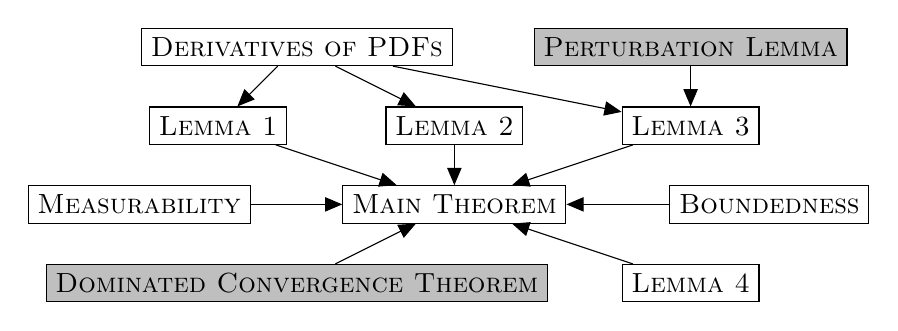
\begin{tikzpicture}
      \node [rectangle, draw, fill=lightgray] (perturbation) at (3, 0) {\textsc{Perturbation Lemma}};
      \node [rectangle, draw, fill=lightgray] (lebesgue) at (-2, -3) {\textsc{Dominated Convergence Theorem}};
      \node [rectangle, draw] (derivatives) at (-2, 0) {\textsc{Derivatives of PDFs}};
      \node [rectangle, draw] (measurability) at (-4, -2) {\textsc{Measurability}};
      \node [rectangle, draw] (boundedness) at (4, -2) {\textsc{Boundedness}};
      \node [rectangle, draw] (lemma1) at (-3, -1) {\textsc{Lemma 1}};
      \node [rectangle, draw] (lemma2) at (0, -1) {\textsc{Lemma 2}};
      \node [rectangle, draw] (lemma3) at (3, -1) {\textsc{Lemma 3}};
      \node [rectangle, draw] (lemma4) at (3, -3) {\textsc{Lemma 4}};
      \node [rectangle, draw] (theorem) at (0, -2) {\textsc{Main Theorem}};
      \draw [->] (perturbation) edge (lemma3);
      \draw [->] (lebesgue) edge (theorem);
      \draw [->] (derivatives) edge (lemma1);
      \draw [->] (derivatives) edge (lemma2);
      \draw [->] (derivatives) edge (lemma3);
      \draw [->] (measurability) edge (theorem);
      \draw [->] (boundedness) edge (theorem);
      \draw [->] (lemma1) edge (theorem);
      \draw [->] (lemma2) edge (theorem);
      \draw [->] (lemma3) edge (theorem);
      \draw [->] (lemma4) edge (theorem);
    \end{tikzpicture}
  \end{figure}
\end{frame}

\begin{frame}{Mathematical Preliminaries}
  \begin{table}
    \centering
    \begin{tabular}{cc}
      Vector norms & Matrix norms \\
      {$\!\begin{aligned}
          \lVert \mathbf{x} \rVert_1 &= \sum_i |x_i| \\
          \lVert \mathbf{x} \rVert_\infty &= \max_i |x_i|
        \end{aligned}$} & {$\!\begin{aligned}
          \lVert \mathbf{A} \rVert_p &= \sup_{\mathbf{x} \ne \mathbf{0}} \frac{\lVert \mathbf{Ax} \rVert_p}{\lVert \mathbf{x} \rVert_p} \\
          \lVert \mathbf{A} \rVert_\infty &= \max_i \sum_{j} |A_{i,j}|
        \end{aligned}$}
    \end{tabular}
  \end{table}
  \begin{lemma}[Perturbation Lemma]
    Let $\lVert \cdot \rVert$ be any matrix norm, and let $\mathbf{A}$ and
    $\mathbf{E}$ be matrices such that $\mathbf{A}$ is invertible and $\lVert
    \mathbf{A}^{-1} \rVert \lVert \mathbf{E} \rVert < 1$, then $\mathbf{A} +
    \mathbf{E}$ is invertible, and
    \[
      \lVert (\mathbf{A} + \mathbf{E})^{-1} \rVert \le \frac{\lVert
        \mathbf{A}^{-1} \rVert}{1 - \lVert \mathbf{A}^{-1} \rVert \lVert
        \mathbf{E} \rVert}.
    \]
  \end{lemma}
\end{frame}

\begin{frame}{Theoretical Results}
  Seeing $V$ as $V : \mathcal{S} \to \mathbb{R}^{|\mathcal{S}|} \to
  \mathbb{R}$... \\~\\

  \begin{proposition}
    MDP value functions $V(s) : \mathbb{R}^{|\mathcal{S}|} \to \mathbb{R}$ (for
    $s \in \mathcal{S}$) are Lebesgue measurable.
  \end{proposition}
  \begin{proposition}
    If the initial values of the MDP value function satisfy the following
    bound, then the bound remains satisfied throughout value iteration:
    \[
      |V_{\mathbf{r}}(s)| \le \vbound.
    \]
  \end{proposition}
\end{frame}

\begin{frame}{Theoretical Results}
  \begin{theorem} \label{thm:main}
    Whenever the derivative exists,
    \[
      \dt\iint
      V_{\mathbf{r}}(s)q(\mathbf{r} \mid \mathbf{u})q(\mathbf{u})\dx
      = \iint
      \dt[V_{\mathbf{r}}(s)q(\mathbf{r} \mid \mathbf{u})q(\mathbf{u})]\dx,
    \]
    where $t$ is any scalar part of $\bm\mu$, $\bm\Sigma$, or $\bm\lambda$.
  \end{theorem}
\end{frame}

\begin{frame}{A Note on Polynomials}
  \begin{definition}
    Let $\mathbb{R}_d[\mathbf{x}]$ denote the vector space of polynomials with
    degree at most $d$, where variables are elements of $\mathbf{x}$, and
    coefficients are in $\mathbb{R}$.
  \end{definition}
  \begin{example}
    \begin{align*}
      2x_1^2 + \pi x_2 &\in \mathbb{R}_2[\mathbf{x}] \\
      x_1x_2 &\in \mathbb{R}_2[\mathbf{x}] \\
      -3x_1 + 1 &\in \mathbb{R}_2[\mathbf{x}] \\
      0 &\in \mathbb{R}_2[\mathbf{x}]
    \end{align*}
  \end{example}
\end{frame}

\begin{frame}{Helpful Lemmas}
  \begin{lemma}
    \[
      \int \lVert \mathbf{r} \rVert_\infty q(\mathbf{r} \mid
      \mathbf{u})\,d\mathbf{r} \le a + \lVert \Kru^\intercal \Kuu^{-1}
      \mathbf{u} \rVert_1,
    \]
    where $a$ is a constant independent of $\mathbf{u}$.
  \end{lemma}
  \begin{lemma}
    Let $c : \mathbb{R}^{|\mathcal{S}|} \times \mathbb{R}^m \to (a, b) \subset
    \mathbb{R}$ be an arbitrary bounded function. Then, for $i = 0,
    \dots, d$,
    \[
      \left. \frac{\partial q(\mathbf{r} \mid \mathbf{u})}{\partial \lambda_i}
      \right|_{\lambda_i = c(\mathbf{r}, \mathbf{u})}
    \]
    has upper and lower bounds of the form $q(\mathbf{r} \mid
    \mathbf{u})d(\mathbf{u})$, where $d(\mathbf{u}) \in
    \mathbb{R}_2[\mathbf{u}]$.
  \end{lemma}
\end{frame}

\begin{frame}{Helpful Lemmas}
  \begin{lemma}
    Let $c : \mathbb{R}^{|\mathcal{S}|} \times \mathbb{R}^m \to (a, b) \subset
    \mathbb{R}$ be an arbitrary bounded function. Then, for $i = 1, \dots, m$,
    every element of
    \[
      \left. \frac{\partial q(\mathbf{u})}{\partial \bm\mu} \right|_{\mu_i =
        c(\mathbf{r}, \mathbf{u})}
    \]
    has upper and lower bounds of the form $q(\mathbf{u})d(\mathbf{u})$,
    where $d(\mathbf{u}) \in \mathbb{R}_1[\mathbf{u}]$.
  \end{lemma}
\end{frame}

\begin{frame}{Helpful Lemmas}
  \begin{lemma} \label{lemma:bound3}
    Let $i, j = 1, \dots, m$, and let $\epsilon > 0$ be arbitrary. Furthermore,
    let
    \[
      c : \mathbb{R}^{|\mathcal{S}|} \times \mathbb{R}^m \to (\Sigma_{i,j} - \epsilon,
      \Sigma_{i,j} + \epsilon) \subset \mathbb{R}
    \]
    be a function with a codomain arbitrarily close to $\Sigma_{i,j}$. Then every
    element of
    \[
      \left. \frac{\partial q(\mathbf{u})}{\partial \bm\Sigma} \right|_{\Sigma_{i,j} =
        c(\mathbf{r}, \mathbf{u})}
    \]
    has upper and lower bounds of the form $q(\mathbf{u})d(\mathbf{u})$, where
    $d(\mathbf{u}) \in \mathbb{R}_2[\mathbf{u}]$.
  \end{lemma}
\end{frame}

\section{Experiments}
% TODO: fix the wording of epsilon in the theorems

\begin{frame}{Experimental Scenario}
  \begin{figure}
    \centering
    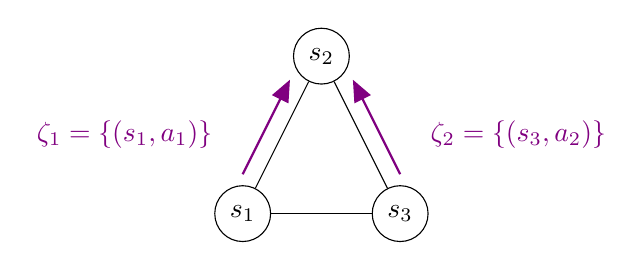
\begin{tikzpicture}
      \node[draw,circle] (s1) at (0, 0) {$s_1$};
      \node[draw,circle] (s2) at (1, 2) {$s_2$};
      \node[draw,circle] (s3) at (2, 0) {$s_3$};
      \draw (s1) to (s2);
      \draw (s1) to (s3);
      \draw (s2) to (s3);
      \draw[->,thick,violet] (0, 0.5) to (0.6, 1.7);
      \draw[->,thick,violet] (2, 0.5) to (1.4, 1.7);
      \node[violet] (label1) at (-1.5, 1.0) {$\zeta_1 = \{ (s_1, a_1) \}$};
      \node[violet] (label2) at (3.5, 1.0) {$\zeta_2 = \{ (s_3, a_2) \}$};
    \end{tikzpicture}
  \end{figure}
\end{frame}

\begin{frame}{Convergence}
  \hspace*{1cm}
  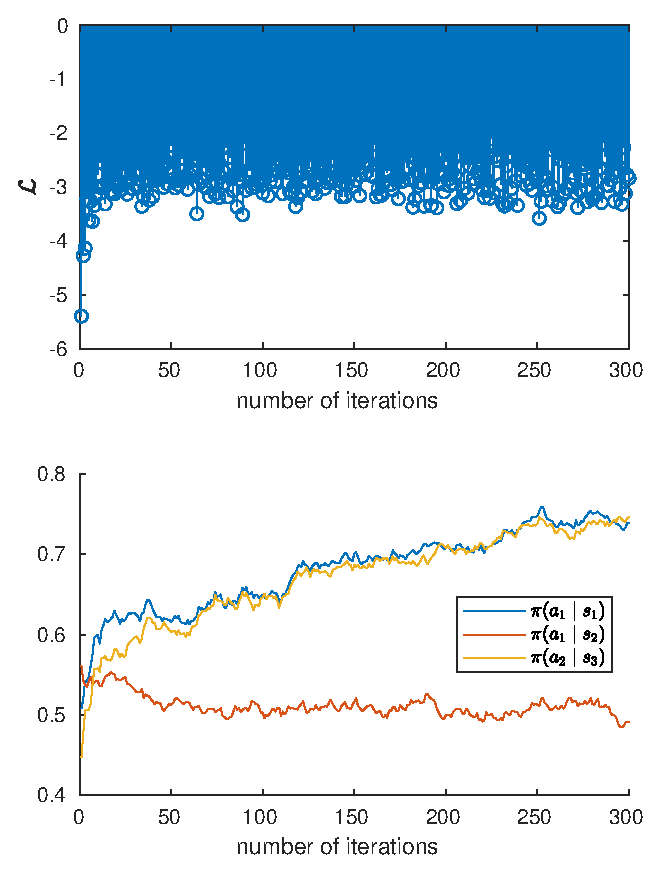
\includegraphics[height=0.8\textheight]{../mpaper/figures/convergence_new}
  \begin{tikzpicture}[remember picture,overlay]
    \begin{scope}[yshift=3cm,xshift=0.5cm]
      \node[draw,circle] (s1) at (0, 0) {$s_1$};
      \node[draw,circle] (s2) at (1, 2) {$s_2$};
      \node[draw,circle] (s3) at (2, 0) {$s_3$};
      \draw[dashed] (s1) to (s2);
      \draw[dashed] (s1) to (s3);
      \draw[dashed] (s2) to (s3);
      \draw[->,mybluetwo,bend left] (s1) to (s2);
      \draw[->,myredtwo,bend left] (s2) to (s1);
      \draw[->,myyellow,bend right] (s3) to (s2);
    \end{scope}
  \end{tikzpicture}
\end{frame}

\begin{frame}{Parameter Convergence}
  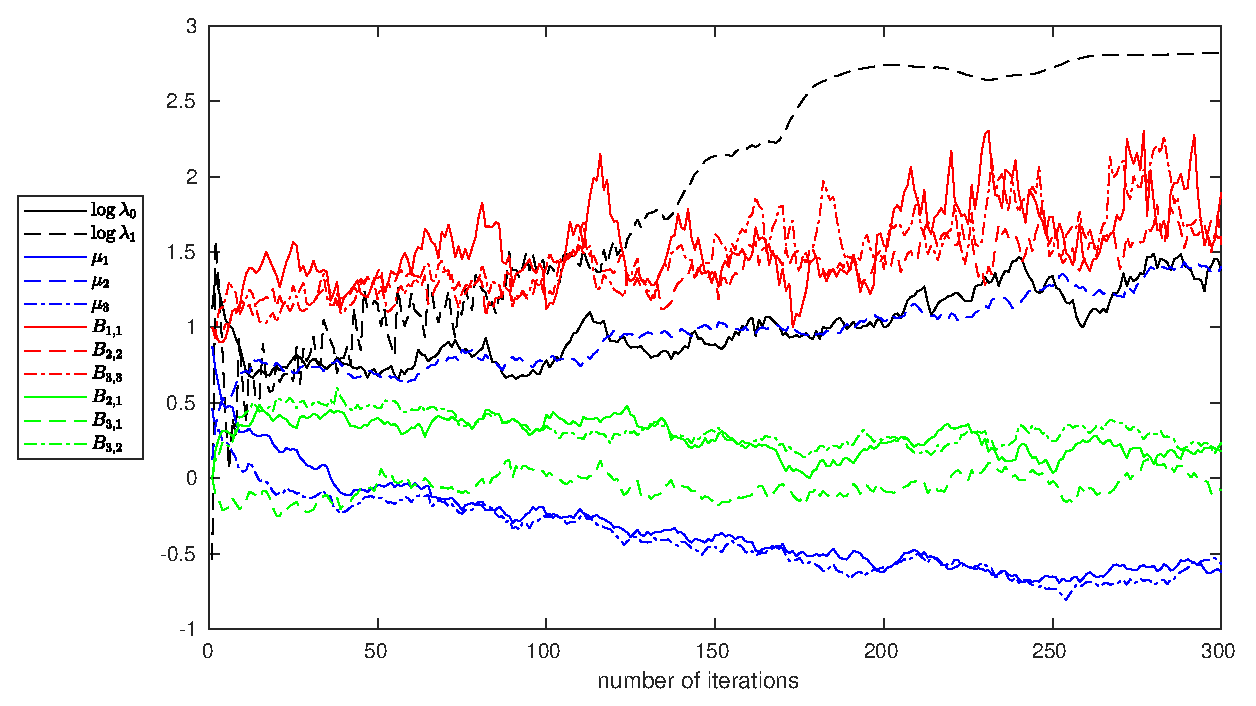
\includegraphics[width=\textwidth]{../mpaper/figures/parameter_convergence_new}
\end{frame}

\begin{frame}{Policy}
  \begin{tikzpicture}
    \csvreader[
    no head,
    column count=11
    ]{../mpaper/data/covariance_and_policy_transformed.csv}{1=\x, 2=\y, 3=\Soneone, 4=\Stwotwo, 5=\Sthreethree, 6=\Stwoone, 7=\Sthreeone, 8=\Sthreetwo, 9=\ponetwo, 10=\ptwoone, 11=\pthreetwo}{%
      \begin{axis}[
        ybar=0,
        symbolic x coords={a,b,c},
        ticks=none,
        ymax=1,
        ymin=0,
        x=20,
        bar width=20,
        enlarge x limits=0.25,
        at={(350*\x, 110*\y)},
        height=100,
        bar shift=0pt,
        legend style={
          legend columns=-1,
          at={(1.7,-0.4)}
        }
        ]
        \addplot coordinates {(a, \ponetwo)};
        \addplot coordinates {(b, \ptwoone)};
        \addplot coordinates {(c, \pthreetwo)};
        \draw[dashed] (-50,50) -- (270,50);
        % \ifthenelse{\x=2 \AND \y=1}{
        % \legend{$\pione$,$\pitwo$,$\pithree$};
        % }{}
      \end{axis}
    }
    \draw [<->] (2.3, 8.5) node (yaxis) [above] {$\zeta_2$}
    |- (10, 2) node (xaxis) [right] {$\zeta_1$};
    \foreach \x in {1, 2, 3} {
      \node (x\x) at (1+2.5*\x, 1.7) {$\x$};
    }
    \foreach \y in {1, 2, 3} {
      \node (y\y) at (2.1, 1+2.1*\y) {$\y$};
    }
    \begin{scope}[yshift=5cm,xshift=10.5cm]
      \node[draw,circle] (s1) at (0, 0) {$s_1$};
      \node[draw,circle] (s2) at (1, 2) {$s_2$};
      \node[draw,circle] (s3) at (2, 0) {$s_3$};
      \draw[dashed] (s1) to (s2);
      \draw[dashed] (s1) to (s3);
      \draw[dashed] (s2) to (s3);
      \draw[->,myblue,bend left] (s1) to (s2);
      \draw[->,myred,bend left] (s2) to (s1);
      \draw[->,mybrown,bend right] (s3) to (s2);
    \end{scope}
  \end{tikzpicture}
\end{frame}

\begin{frame}{Covariance: Attempt 1}
  \begin{figure}
    \centering
  \begin{tikzpicture}[
    /pgfplots/colormap/violet,
    ellipse2/.style={
      draw,
      circle,
      /utils/exec={
        \pgfplotscolormapdefinemappedcolor{####1}},
      fill=mapped color},
    edge2/.style={
      ultra thick,
      /utils/exec={
        \pgfplotscolormapdefinemappedcolor{####1}},
      draw=mapped color}]
    \csvreader[
    no head,
    column count=11
    ]{../mpaper/data/median_covariance_transformed.csv}{1=\x, 2=\y, 3=\Soneone, 4=\Stwotwo, 5=\Sthreethree, 6=\Stwoone, 7=\Sthreeone, 8=\Sthreetwo}{%
      \node[ellipse2=\Soneone] (s1) at (2*\x, 2*\y) {$s_1$};
      \node[ellipse2=\Stwotwo] (s2) at (2*\x+0.5, 2*\y+1) {$s_2$};
      \node[ellipse2=\Sthreethree] (s3) at (2*\x+1, 2*\y) {$s_3$};
      \draw[edge2=\Stwoone] (s1) -- (s2);
      \draw[edge2=\Sthreeone] (s1) to (s3);
      \draw[edge2=\Sthreetwo] (s2) to (s3);
    }
    \draw [<->] (1.5, 7.5) node (yaxis) [above] {$\zeta_2$}
    |- (8, 1.5) node (xaxis) [right] {$\zeta_1$};
    \foreach \x in {1, 2, 3} {
      \draw[shift={(0.5+2*\x, 1.5)}] (0pt,2pt) -- (0pt,-2pt) node[below] {$\x$};
    }
    \foreach \y in {1, 2, 3} {
      \draw[shift={(1.5, 0.5+2*\y)}] (2pt,0pt) -- (-2pt,0pt) node[left] {$\y$};
    }
    \begin{axis}[
      colormap/violet,
      scale only axis,
      width=0pt,
      height=0pt,
      hide axis,
      colorbar,
      point meta min=-1,
      point meta max=1,
      xshift=250,
      yshift=210,
      colorbar style={
        height=6cm,
        ytick={-1,0,1},
        ylabel=normalised covariance,
        ylabel style={
          yshift=-1cm
        }
      }]
      \addplot [draw=none] coordinates {(0,0)};
    \end{axis}
  \end{tikzpicture}
  \end{figure}
\end{frame}

\begin{frame}{Covariance: Attempt 2 (with Cliques!)}
  \begin{figure}
    \centering
    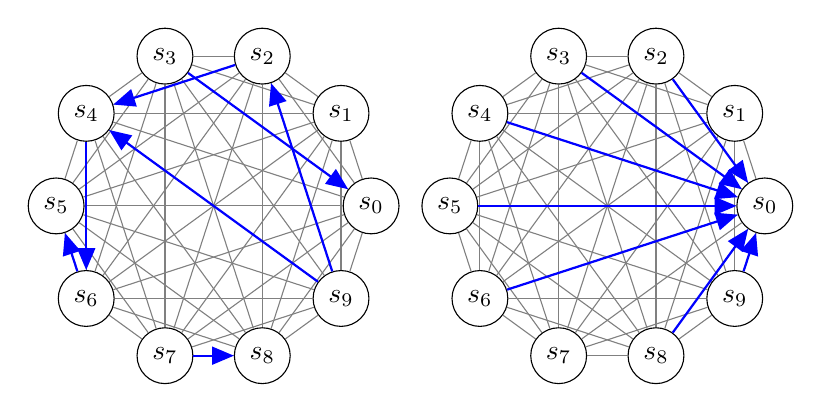
\begin{tikzpicture}
      \foreach \i in {0,...,9}
      \node[draw,circle] (v\i) at (360/10 * \i:2cm) {$s_{\i}$};
      \foreach \i in {0,...,9}
      \foreach \j in {0,...,\i}
      \draw[gray] (v\i) -- (v\j);

      \only<2>{
        \draw[->,thick,blue] (v9) -- (v2);
        \draw[->,thick,blue] (v7) -- (v8);
        \draw[->,thick,blue] (v9) -- (v4);
        \draw[->,thick,blue] (v3) -- (v0);
        \draw[->,thick,blue] (v2) -- (v4);
        \draw[->,thick,blue] (v4) -- (v6);
        \draw[->,thick,blue] (v6) -- (v5);
      }

      \begin{scope}[xshift=5cm]
        \foreach \i in {0,...,9}
        \node[draw,circle] (v\i) at (360/10 * \i:2cm) {$s_{\i}$};
        \foreach \i in {0,...,9}
        \foreach \j in {0,...,\i}
        \draw[gray] (v\i) -- (v\j);

        \only<2>{
          \draw[->,thick,blue] (v3) -- (v0);
          \draw[->,thick,blue] (v4) -- (v0);
          \draw[->,thick,blue] (v6) -- (v0);
          \draw[->,thick,blue] (v2) -- (v0);
          \draw[->,thick,blue] (v5) -- (v0);
          \draw[->,thick,blue] (v8) -- (v0);
          \draw[->,thick,blue] (v9) -- (v0);
        }
      \end{scope}
    \end{tikzpicture}
  \end{figure}
\end{frame}

\begin{frame}{Covariance: Attempt 2 (with Cliques!)}
\begin{figure}
  \centering
  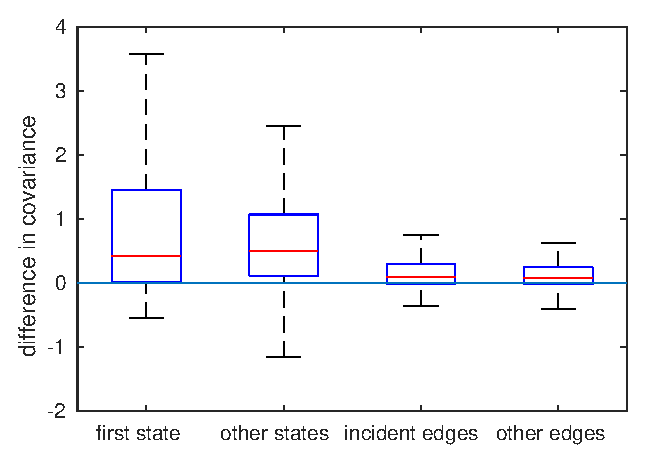
\includegraphics[width=\columnwidth]{../mpaper/figures/boxplots}
\end{figure}
\end{frame}

\section{Conclusion}

% TODO: slide for conclusions:
% 1. we proved that we can
% 2. we showed some other theoretical results
% 3. we showed correctness (both actual predictions and covariances)
% 4. we opened up many new research opportunities

\begin{frame}{Further Work}
  \begin{minipage}[t]{\textwidth}
    \begin{columns}[t]
      \begin{column}{0.9\textwidth}
        \begin{itemize}
        \item More flexible models using...
          \begin{itemize}
          \item normalizing flows\footfullcite{DBLP:conf/icml/RezendeM15}
          \item spectral kernels\footfullcite{pmlr-v28-wilson13}
          \end{itemize}
        \item Faster GP inference and MDP solving
        \item IRL in the context of reinforcement learning
        \item Interplay between rewards and stochastic/deterministic policies
        \end{itemize}
        \vspace{1.5cm}
      \end{column}
      \begin{column}{0.1\textwidth}
        \vspace{-1cm}
        \begin{figure}
          \centering
          
\includegraphics[scale=0.1]{images/flows-1.png}

          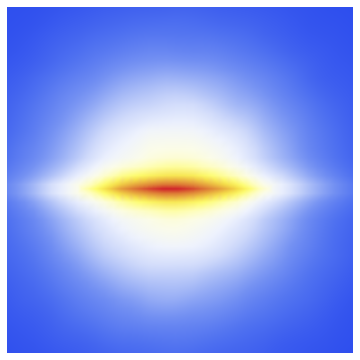
\includegraphics[scale=0.1]{images/flows-2.png}

          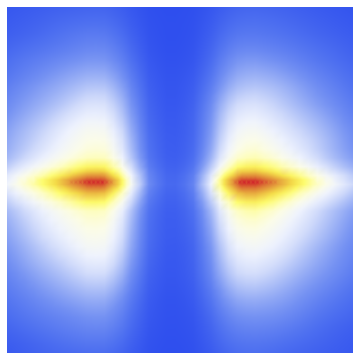
\includegraphics[scale=0.1]{images/flows-3.png}

          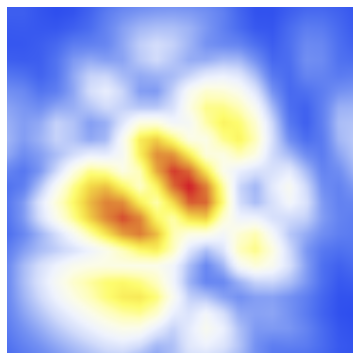
\includegraphics[scale=0.1]{images/flows-4.png}
        \end{figure}
      \end{column}
    \end{columns}
    \pause
    \begin{tikzpicture}[remember picture,overlay]
      \node at (0.5\textwidth, 2.5) {\large\emph{Thank You!}};
    \end{tikzpicture}
  \end{minipage}
\end{frame}

\end{document}